\chapter{Results}
\label{sec:results}
This chapter shows the results obtained from the training phase of the two networks and from the execution of the three experiments described in chapter~\ref{ch:experiment}. After that, the chapter provides a detailed discussion of the proposed results. In particular, Section~\ref{sec:results-training} shows the graphs of the two networks losses and the sample evaluation metrics described in chapter~\ref{ch:system_design}. Section~\ref{sec:results-experiments} shows the test outcomes for the three experiments we conducted. Section~\ref{sec:samples} shows a set of levels sampled from both networks. Section \ref{sec:results-evaluation} provides our discussion on the results by considering them in the same order they are presented. 

\section{Training and Sample Metrics}
\label{sec:results-training}
\paragraph{} In this section we show the metrics that are calculated during the training phase of each network, including the losses and the Sample Evaluation Metrics described in section~\ref{sec:evaluation}. Figures \ref{fig:train-uncond-loss} and \ref{fig:train-cond-loss} show the training and validation loss for the unconditional and conditional networks, respectively. For each feature map, Figures from~\ref{fig:train-entropy-mean} to \ref{fig:train-entropy-thingsmap} show the Entropy Mean Absolute Error, Figure \ref{fig:train-similarity} shows the Structural Similarity, Figures from~\ref{fig:train-encoding_error-floormap} to~\ref{fig:train-encoding-error-thingsmap} show the Encoding Error, Figure~\ref{fig:floor_corner_error} and \ref{fig:wall_corner_error} show the Corner Error for the FloorMap and WallMap, respectively.

\begin{figure}[!htb] 
	\begin{minipage}[b]{0.9\linewidth}
		\centering
		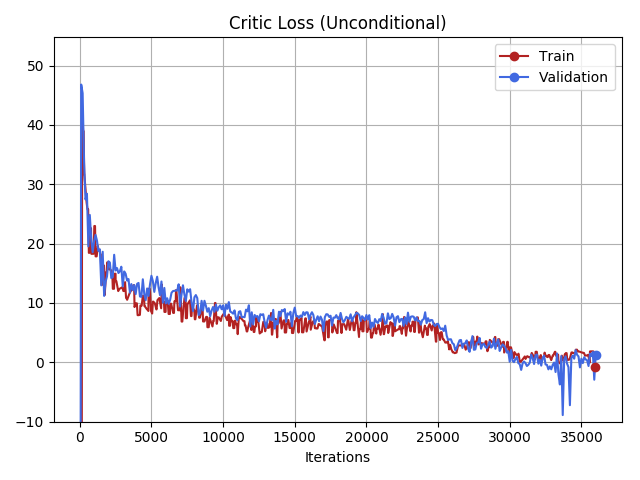
\includegraphics[width=\linewidth]{results/train/uncond_loss.png} 
		\caption[Unconditional Network Loss]{Unconditional Network Loss for the Critic: Training loss (red) and Validation Loss (blue) both converge toward zero.}
		\label{fig:train-uncond-loss}
	\end{minipage}
	
	\begin{minipage}[b]{0.9\linewidth}
	\centering
	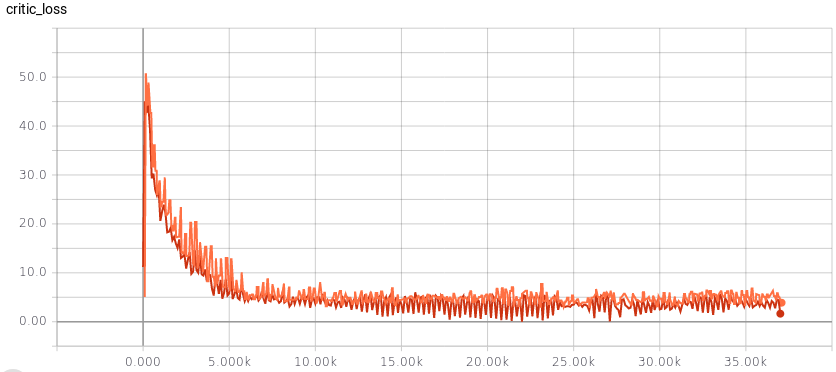
\includegraphics[width=\linewidth]{results/train/cond_loss.png} 
	\caption[Conditional Network Loss]{Conditional Network Loss for the Critic: Training loss (Red) and Validation Loss (Blue) both converge toward zero.}
	\label{fig:train-cond-loss}
\end{minipage}
\end{figure}

\begin{figure}[!htb] 
	\begin{minipage}[b]{0.9\linewidth}
		\centering
		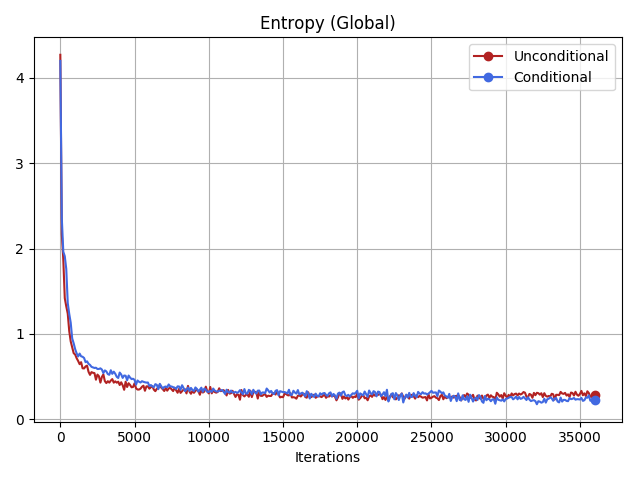
\includegraphics[width=\linewidth]{results/train/entropy.png} 
		\caption[Sample Evaluation Metrics: Entropy] {Sample Evaluation Metrics: Mean Entropy difference over all the maps (floormap, wallmap, thingsmap, heightmap). Unconditional (Red) and Conditional (Blue) networks generate samples having similar mean entropy. }
		\label{fig:train-entropy-mean}
	\end{minipage}
\end{figure}

\begin{figure}[!htb] 
	\begin{minipage}[t]{0.45\linewidth}
	\centering
	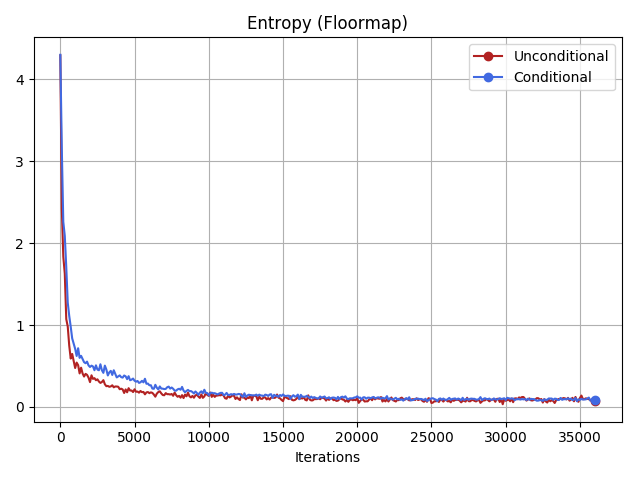
\includegraphics[width=\linewidth]{results/train/entropy_floormap.png} 
	\caption[Sample Evaluation Metrics: Entropy (Floormap)]{Sample Evaluation Metrics: Entropy MAE calculated on FloorMap. Unconditional (Red) and Conditional (Blue) networks generate samples having similar Floormap entropy.}
	\label{fig:train-entropy-floormap}
\end{minipage}
\hfil
\begin{minipage}[t]{0.45\linewidth}
	\centering
	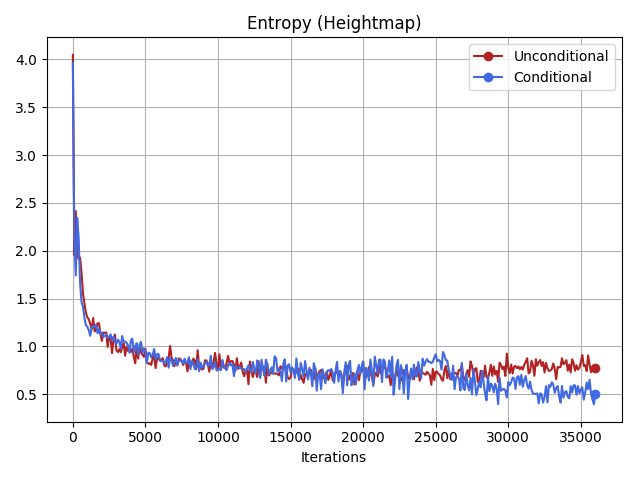
\includegraphics[width=\linewidth]{results/train/entropy_heightmap.png} 
	\caption[Sample Evaluation Metrics: Entropy (HeightMap)]{Sample Evaluation Metrics: Entropy MAE calculated on HeightMap. Conditional (Blue) network generate samples having slightly better HeightMap entropy than the Unconditional network (Red).}
	\label{fig:train-entropy-heightmap}
\end{minipage}

\begin{minipage}[t]{0.45\linewidth}
	\centering
	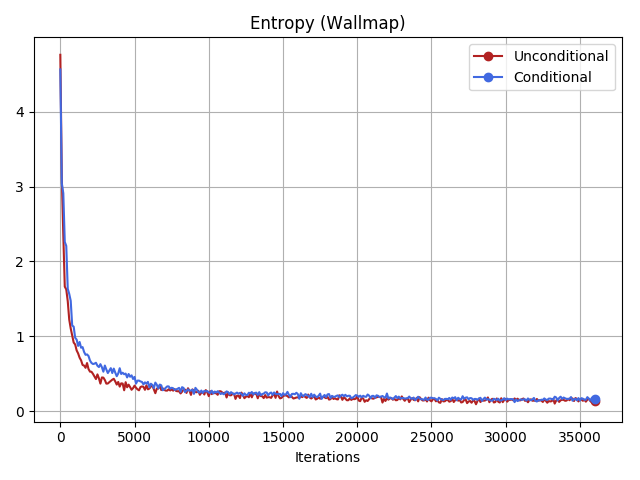
\includegraphics[width=\linewidth]{results/train/entropy_wallmap.png} 
	\caption[Sample Evaluation Metrics: Entropy (WallMap)]{Sample Evaluation Metrics: Entropy MAE calculated on WallMap. Unconditional (Red) and Conditional (Blue) networks generate samples having similar WallMap entropy.}
	\label{fig:train-entropy-wallmap}
\end{minipage}
\hfil
\begin{minipage}[t]{0.45\linewidth}
	\centering
	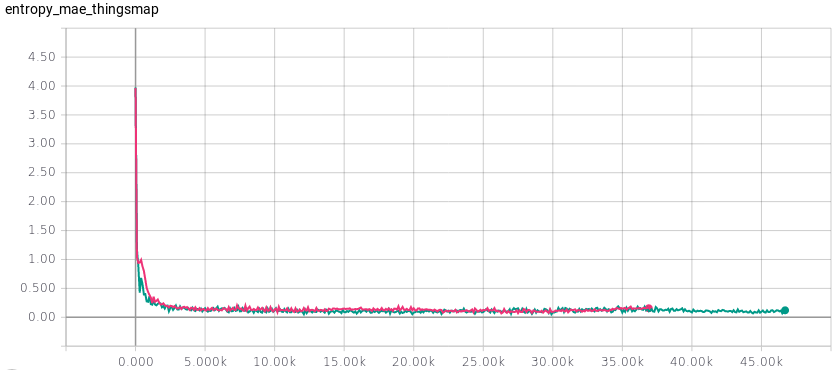
\includegraphics[width=\linewidth]{results/train/entropy_thingsmap.png} 
	\caption[Sample Evaluation Metrics: Entropy (ThingsMap)]{Sample Evaluation Metrics: Entropy MAE calculated on ThingsMap. Unconditional (Red) and Conditional (Blue) networks generate samples having similar ThingsMap entropy.}
	\label{fig:train-entropy-thingsmap}
\end{minipage}
\end{figure}

\begin{figure}[!htb] 
	\begin{minipage}[b]{\linewidth}
		\centering
		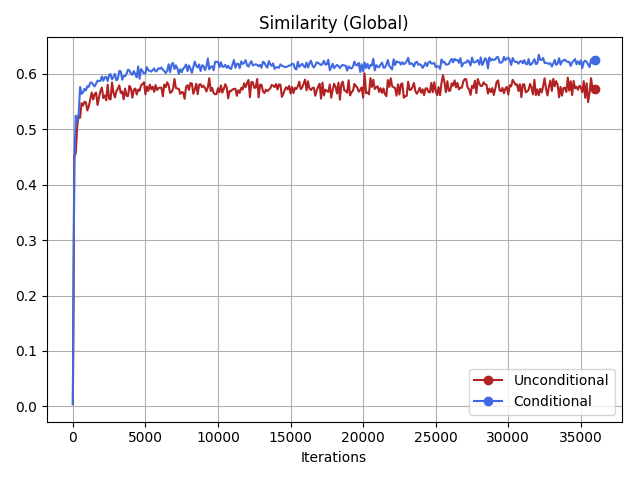
\includegraphics[width=\linewidth]{results/train/similarity.png} 
		\caption[Sample Evaluation Metrics: Mean Structural Similarity Index]{Sample Evaluation Metrics: Mean Structural Similarity over the samples. Conditional (Blue) networks generate samples being more similar to true ones than the Unconditional network (Red).}
		\label{fig:train-similarity}
	\end{minipage}
\end{figure}


\begin{figure}[!htb] 
	\begin{minipage}[t]{0.45\linewidth}
		\centering
		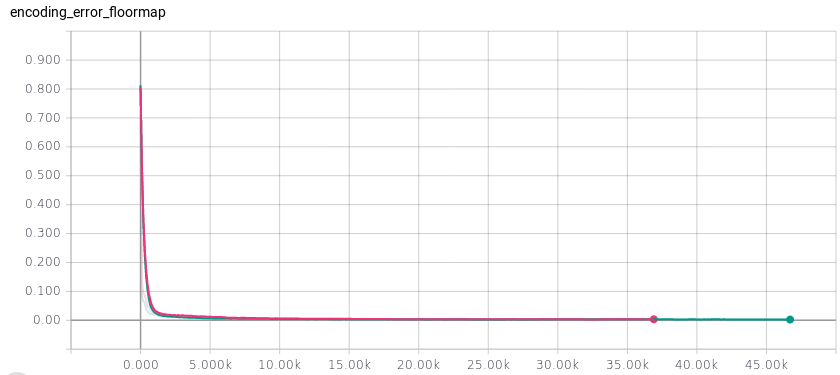
\includegraphics[width=\linewidth]{results/train/encoding_error_floormap.png} 
		\caption[Sample Evaluation Metrics: Encoding Error (Floormap)]{Sample Evaluation Metrics: Encoding Error calculated on FloorMap. Both Unconditional (Red) and Conditional (Blue) networks learns the colour scheme for representing the floors.}
		\label{fig:train-encoding_error-floormap}
	\end{minipage}
	\hfil
	\begin{minipage}[t]{0.45\linewidth}
		\centering
		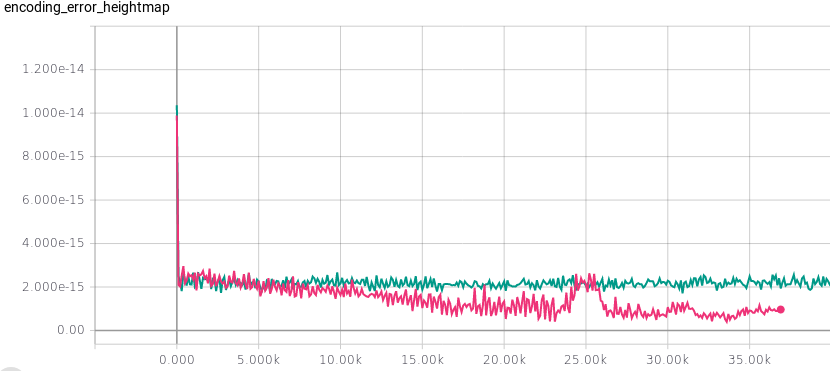
\includegraphics[width=\linewidth]{results/train/encoding_error_heightmap.png} 
		\caption[Sample Evaluation Metrics: Encoding Error (HeightMap)]{Sample Evaluation Metrics: Encoding Error calculated on HeightMap. Conditional (Blue) network is slightly more precise in representing the colour coding for the floor height than the Unconditional network (Red).}
		\label{fig:train-encoding-error-heightmap}
	\end{minipage}
	
	\begin{minipage}[t]{0.45\linewidth}
		\centering
		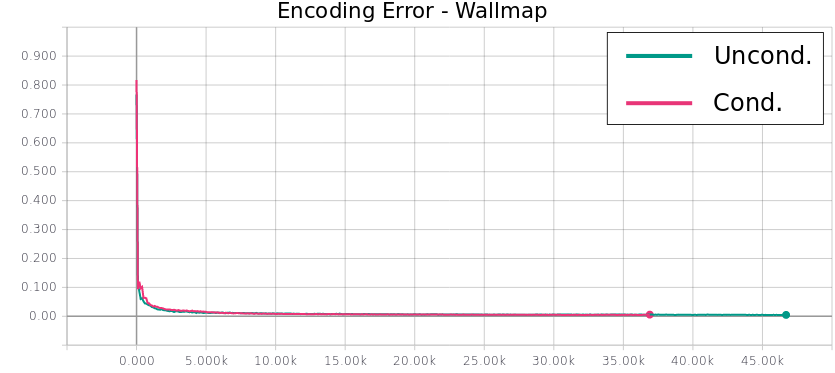
\includegraphics[width=\linewidth]{results/train/encoding_error_wallmap.png} 
		\caption[Sample Evaluation Metrics: Encoding Error (WallMap)]{Sample Evaluation Metrics: Encoding Error calculated on WallMap. Both Unconditional (Red) and Conditional (Blue) networks learns the colour scheme for representing the walls.}
		\label{fig:train-encoding-error-wallmap}
	\end{minipage}
	\hfil
	\begin{minipage}[t]{0.45\linewidth}
		\centering
		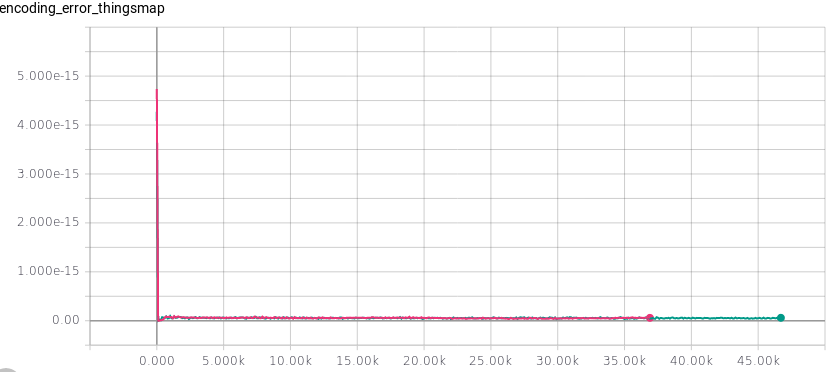
\includegraphics[width=\linewidth]{results/train/encoding_error_thingsmap.png} 
		\caption[Sample Evaluation Metrics: Encoding Error (ThingsMap)]{Sample Evaluation Metrics: Encoding Error calculated on ThingsMap. Both Unconditional (Red) and Conditional (Blue) networks learns the colour scheme for representing the game objects.}
		\label{fig:train-encoding-error-thingsmap}
	\end{minipage}
\end{figure}

\begin{figure}[!htb] 
	\begin{minipage}[b]{0.9\linewidth}
		\centering
		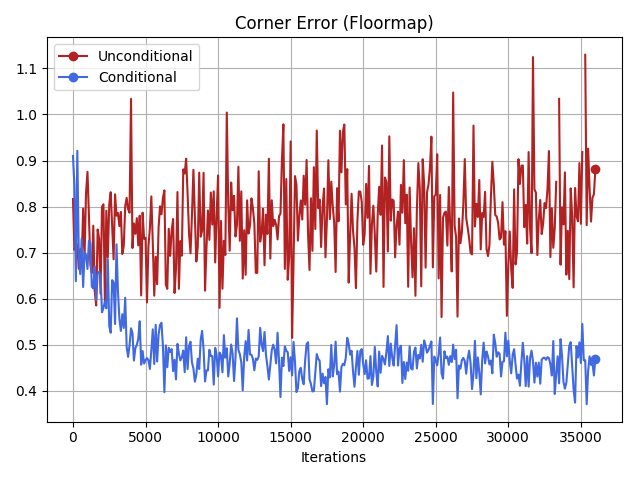
\includegraphics[width=\linewidth]{results/train/floor_corner_error.png} 
		\caption[Sample Evaluation Metrics: Mean Corner Error (FloorMap)]{Sample Evaluation Metrics: Mean Corner Error over the FloorMap. Conditional (Blue) networks generate samples having a floor corner count closer to true levels than the Unconditional network (Red).}
		\label{fig:floor_corner_error}
	\end{minipage}

	\begin{minipage}[b]{0.9\linewidth}
		\centering
		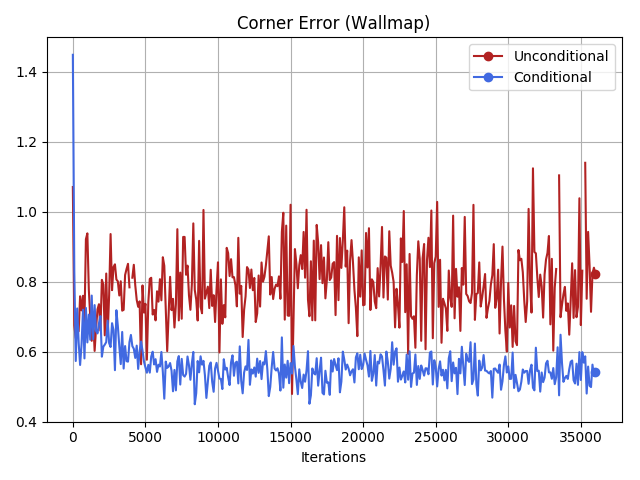
\includegraphics[width=\linewidth]{results/train/walls_corner_error.png} 
		\caption[Sample Evaluation Metrics: Mean Corner Error (WallMap)]{Sample Evaluation Metrics: Mean Corner Error over the WallMap. Conditional (Blue) networks generate samples having a wall corner count closer to true levels than the Unconditional network (Red).}
		\label{fig:wall_corner_error}
	\end{minipage}
\end{figure}


\FloatBarrier
\section{Experiment Results}
\label{sec:results-experiments}
\paragraph{} This section presents the test results for experiment 1 and 2, and the graphs produced by the experiment 3.
\subsection{Results of experiments 1 and 2}
\paragraph{} Results for experiments 1 and 2 are shown respectively in the first two columns of Table~\ref{tab:results-input-features} and \ref{tab:results-other-features}. The third column indicates the feature group according to the description made in section \ref{sec:experiment-2}. The set of features is divided in input and non-input features, with reference to the conditional network.
	
	\subsubsection{Input Features}
	\begin{longtable}{llll}
		\caption[Test results for input features]{ \small KS-test results for input features, using a significance level of 0.05 and the Bonferroni correction method. Results are indicated with R if the null hypothesis can be rejected or with N otherwise. An asterisk indicates the network that performed better (has the minimum KS distance) if the null hypothesis is rejected in every network}\\
		\toprule
		{} & uncond & cond & Group \\
		feature                   &        &      &       \\
		\midrule
		\endhead
		\midrule
		\multicolumn{3}{r}{{Continued on next page}} \\
		\midrule
		\endfoot
		
		\bottomrule
		\endlastfoot
		level\_equivalent\_diameter &      N &    N &    F3 \\
		level\_major\_axis\_length   &     R* &    R &    F1 \\
		level\_minor\_axis\_length   &      N &    N &    F3 \\
		level\_solidity            &      R &   R* &    F1 \\
		nodes                     &      R &   R* &    F1 \\
		distmap-skew              &      R &   R* &    F1 \\
		distmap-kurt              &      R &    N &    F2 \\
		\label{tab:results-input-features}
	\end{longtable}
	
	
	\subsubsection{Non-Input Features}	
	
	\begin{longtable}{llll}
		\caption[Test results for non input features]{ \small KS-test results for non-input features, using a significance level of 0.05 and the Bonferroni correction method. Results are indicated with R if the null hypothesis can be rejected or with N otherwise. An asterisk indicates the network that performed better (has the minimum KS distance) if the null hypothesis is rejected in every network}\\
		\toprule
		{} & uncond & cond & Group \\
		feature                       &        &      &       \\
		\midrule
		\endhead
		\midrule
		\multicolumn{3}{r}{{Continued on next page}} \\
		\midrule
		\endfoot
		
		\bottomrule
		\endlastfoot
		level\_area                    &      N &    N &    F3 \\
		level\_convex\_area             &      N &    N &    F3 \\
		level\_eccentricity            &     R* &    R &    F1 \\
		level\_euler\_number            &      R &   R* &    F1 \\
		level\_extent                  &      R &   R* &    F1 \\
		level\_filled\_area             &      N &    N &    F3 \\
		level\_orientation             &      N &    N &    F3 \\
		level\_perimeter               &      N &    N &    F3 \\
		level\_hu\_moment\_0             &      N &    R &    F4 \\
		level\_hu\_moment\_1             &     R* &    R &    F1 \\
		level\_hu\_moment\_2             &      R &   R* &    F1 \\
		level\_hu\_moment\_3             &      R &    N &    F2 \\
		level\_hu\_moment\_4             &      N &    R &    F4 \\
		level\_hu\_moment\_5             &      N &    R &    F4 \\
		level\_hu\_moment\_6             &      R &    N &    F2 \\
		level\_centroid\_x              &     R* &    R &    F1 \\
		level\_centroid\_y              &     R* &    R &    F1 \\
		number\_of\_artifacts           &      R &   R* &    F1 \\
		number\_of\_powerups            &      R &    N &    F2 \\
		number\_of\_weapons             &      R &   R* &    F1 \\
		number\_of\_ammunitions         &     R* &    R &    F1 \\
		number\_of\_keys                &      R &   R* &    F1 \\
		number\_of\_monsters            &     R* &    R &    F1 \\
		number\_of\_obstacles           &      R &   R* &    F1 \\
		number\_of\_decorations         &      R &   R* &    F1 \\
		walkable\_area                 &      N &    N &    F3 \\
		walkable\_percentage           &      N &    N &    F3 \\
		start\_location\_x\_px           &      R &   R* &    F1 \\
		start\_location\_y\_px           &      R &   R* &    F1 \\
		artifacts\_per\_walkable\_area   &      R &   R* &    F1 \\
		powerups\_per\_walkable\_area    &      R &    N &    F2 \\
		weapons\_per\_walkable\_area     &      R &   R* &    F1 \\
		ammunitions\_per\_walkable\_area &     R* &    R &    F1 \\
		keys\_per\_walkable\_area        &      R &   R* &    F1 \\
		monsters\_per\_walkable\_area    &      R &   R* &    F1 \\
		obstacles\_per\_walkable\_area   &      R &   R* &    F1 \\
		decorations\_per\_walkable\_area &      R &   R* &    F1 \\
		avg-path-length               &      R &   R* &    F1 \\
		diameter-mean                 &      R &   R* &    F1 \\
		art-points                    &     R* &    R &    F1 \\
		assortativity-mean            &     R* &    R &    F1 \\
		betw-cen-min                  &      N &    N &    F3 \\
		betw-cen-max                  &      R &   R* &    F1 \\
		betw-cen-mean                 &     R* &    R &    F1 \\
		betw-cen-var                  &     R* &    R &    F1 \\
		betw-cen-skew                 &      R &   R* &    F1 \\
		betw-cen-kurt                 &      R &   R* &    F1 \\
		betw-cen-Q1                   &     R* &    R &    F1 \\
		betw-cen-Q2                   &     R* &    R &    F1 \\
		betw-cen-Q3                   &     R* &    R &    F1 \\
		closn-cen-min                 &     R* &    R &    F1 \\
		closn-cen-max                 &      R &   R* &    F1 \\
		closn-cen-mean                &     R* &    R &    F1 \\
		closn-cen-var                 &      R &   R* &    F1 \\
		closn-cen-skew                &     R* &    R &    F1 \\
		closn-cen-kurt                &     R* &    R &    F1 \\
		closn-cen-Q1                  &     R* &    R &    F1 \\
		closn-cen-Q2                  &      R &   R* &    F1 \\
		closn-cen-Q3                  &      R &   R* &    F1 \\
		distmap-max                   &     R* &    R &    F1 \\
		distmap-mean                  &     R* &    R &    F1 \\
		distmap-var                   &     R* &    R &    F1 \\
		distmap-Q1                    &     R* &    R &    F1 \\
		distmap-Q2                    &      R &   R* &    F1 \\
		distmap-Q3                    &      R &   R* &    F1 \\
		\label{tab:results-other-features}
	\end{longtable}

\subsection{Graphical results for Experiments 1 and 2}
\paragraph{} Figure~\ref{fig:results-input-features} shows the cumulative distribution functions relative to the features considered in table~\ref{tab:results-input-features}. Another view of the same data is proposed in figure~\ref{fig:results-input-distr-features} in which the probability densities for the input features are shown.

\begin{figure}[h!] 
    \begin{minipage}[b]{0.45\linewidth}
	\centering
	\includegraphics[width=\linewidth]{results/exp1-2/level_equivalent_diameter.pdf} 
	\label{fig:results-input-level_equivalent_diameter}
	\end{minipage}
	\hfil
    \begin{minipage}[b]{0.45\linewidth}
	\centering
	\includegraphics[width=\linewidth]{results/exp1-2/level_solidity.pdf} 
	\label{fig:results-input-level_solidity}
	\end{minipage}

    \begin{minipage}[b]{0.45\linewidth}
	\centering
	\includegraphics[width=\linewidth]{results/exp1-2/level_major_axis_length.pdf} 
	\label{fig:results-input-level_major_axis_length}
\end{minipage}
\hfil
\begin{minipage}[b]{0.45\linewidth}
	\centering
	\includegraphics[width=\linewidth]{results/exp1-2/level_minor_axis_length.pdf} 
	\label{fig:results-input-level_minor_axis_length}
\end{minipage}

    \begin{minipage}[b]{0.45\linewidth}
	\centering
	\includegraphics[width=\linewidth]{results/exp1-2/distmap-skew.pdf} 
	\label{fig:results-input-distmap-skew}
\end{minipage}
\hfil
\begin{minipage}[b]{0.45\linewidth}
	\centering
	\includegraphics[width=\linewidth]{results/exp1-2/distmap-kurt.pdf} 
	\label{fig:results-input-distmap-kurt}
\end{minipage}

	\centering
	\begin{minipage}[b]{0.45\linewidth}
		\centering
		\includegraphics[width=\linewidth]{results/exp1-2/nodes.pdf} 
		\label{fig:results-input-nodes}
	\end{minipage}


\caption[Graphical results for experiments 1 and 2: Cumulative Distributions]{Experiments 1 and 2: Cumulative distribution functions for true data, unconditional network and conditional network for each input feature.}
\label{fig:results-input-features}
\end{figure}

\begin{figure}[h!] 
	\begin{minipage}[b]{0.45\linewidth}
		\centering
		\includegraphics[width=\linewidth]{results/exp1-2/distr/level_equivalent_diameter.pdf} 
		\label{fig:results-input-distr-level_equivalent_diameter}
	\end{minipage}
	\hfil
	\begin{minipage}[b]{0.45\linewidth}
		\centering
		\includegraphics[width=\linewidth]{results/exp1-2/distr/level_solidity.pdf} 
		\label{fig:results-input-distr-level_solidity}
	\end{minipage}
	
	\begin{minipage}[b]{0.45\linewidth}
		\centering
		\includegraphics[width=\linewidth]{results/exp1-2/distr/level_major_axis_length.pdf} 
		\label{fig:results-input-distr-level_major_axis_length}
	\end{minipage}
	\hfil
	\begin{minipage}[b]{0.45\linewidth}
		\centering
		\includegraphics[width=\linewidth]{results/exp1-2/distr/level_minor_axis_length.pdf} 
		\label{fig:results-input-distr-level_minor_axis_length}
	\end{minipage}
	
	\begin{minipage}[b]{0.45\linewidth}
		\centering
		\includegraphics[width=\linewidth]{results/exp1-2/distr/distmap-skew.pdf} 
		\label{fig:results-input-distr-distmap-skew}
	\end{minipage}
	\hfil
	\begin{minipage}[b]{0.45\linewidth}
		\centering
		\includegraphics[width=\linewidth]{results/exp1-2/distr/distmap-kurt.pdf} 
		\label{fig:results-input-distr-distmap-kurt}
	\end{minipage}
	
	\centering
	\begin{minipage}[b]{0.45\linewidth}
		\centering
		\includegraphics[width=\linewidth]{results/exp1-2/distr/nodes.pdf} 
		\label{fig:results-input-distr-nodes}
	\end{minipage}
	
	\caption[Graphical results for experiments 1 and 2: Probability Densities]{Experiments 1 and 2: Estimated probability density functions for true data, unconditional network and conditional network for each input feature.}
	\label{fig:results-input-distr-features}
	
\end{figure}

\FloatBarrier
\subsection{Results of Experiment 3}
\paragraph{} Results of Experiment 3 are shown in figure~\ref{fig:results-exp3-features}. Each figure shows a different input feature. The three vertical lines correspond to the values of the three quartiles that have been used to generate the three distributions of 1000 levels each. 

\begin{figure}[h!] 
	\begin{minipage}[b]{0.45\linewidth}
		\centering
		\includegraphics[width=\linewidth]{results/exp3/level_equivalent_diameter.pdf} 
		\label{fig:results-exp3-level_equivalent_diameter}
	\end{minipage}
	\hfil
	\begin{minipage}[b]{0.45\linewidth}
		\centering
		\includegraphics[width=\linewidth]{results/exp3/level_solidity.pdf} 
		\label{fig:results-exp3-level_solidity}
	\end{minipage}
	
	\begin{minipage}[b]{0.45\linewidth}
		\centering
		\includegraphics[width=\linewidth]{results/exp3/level_major_axis_length.pdf} 
		\label{fig:results-exp3-level_major_axis_length}
	\end{minipage}
	\hfil
	\begin{minipage}[b]{0.45\linewidth}
		\centering
		\includegraphics[width=\linewidth]{results/exp3/level_minor_axis_length.pdf} 
		\label{fig:results-exp3-level_minor_axis_length}
	\end{minipage}
	
	\begin{minipage}[b]{0.45\linewidth}
		\centering
		\includegraphics[width=\linewidth]{results/exp3/distmap-skew.pdf} 
		\label{fig:results-exp3-distmap-skew}
	\end{minipage}
	\hfil
	\begin{minipage}[b]{0.45\linewidth}
		\centering
		\includegraphics[width=\linewidth]{results/exp3/distmap-kurt.pdf} 
		\label{fig:results-exp3-distmap-kurt}
	\end{minipage}
	
	\centering
	\begin{minipage}[b]{0.45\linewidth}
		\centering
		\includegraphics[width=\linewidth]{results/exp3/nodes.pdf} 
		\label{fig:results-exp3-nodes}
	\end{minipage}

	
	\caption[Graphical results for experiments 3: Generated features distribution vs true percentiles]{Experiments 3: Generated distributions for each true feature value in the cases of 25th (red, circles), 50th (green, squares) and 75th (blue, diamonds) percentiles.}
	\label{fig:results-exp3-features}
\end{figure}

\section{Generated Samples}
\label{sec:samples}
\paragraph{} In this section we show a small set of samples that have been generated by the two networks using the "dataset" sampling approach introduced in section \ref{sec:usecase_sampling}. Figures \ref{fig:samples-uncond-1} and \ref{fig:samples-uncond-2} show samples from the unconditional network, one level per row. Figures \ref{fig:samples-cond-1} and \ref{fig:samples-cond-2} show samples from the conditional network and the true levels that correspond to the input feature vector used to sample the network. 
\subsection{Unconditional Network}
\begin{figure}[h!] 
\begin{minipage}[b]{\linewidth}
	\begin{center}
		
\includegraphics[width=2cm]{figures/results/samples/uncond/sample13_map_floormap_generated.png}
		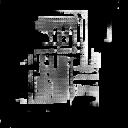
\includegraphics[width=2cm]{figures/results/samples/uncond/sample13_map_heightmap_generated.png}
		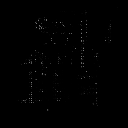
\includegraphics[width=2cm]{figures/results/samples/uncond/sample13_map_thingsmap_generated.png}
		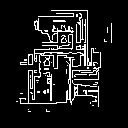
\includegraphics[width=2cm]{figures/results/samples/uncond/sample13_map_wallmap_generated.png}
	\end{center}
	
	\begin{center}
		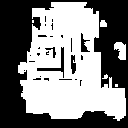
\includegraphics[width=2cm]{figures/results/samples/uncond/sample17_map_floormap_generated.png}
		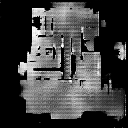
\includegraphics[width=2cm]{figures/results/samples/uncond/sample17_map_heightmap_generated.png}
		
\includegraphics[width=2cm]{figures/results/samples/uncond/sample17_map_thingsmap_generated.png}
		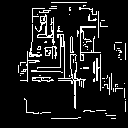
\includegraphics[width=2cm]{figures/results/samples/uncond/sample17_map_wallmap_generated.png}
	\end{center}
	
	\begin{center}
		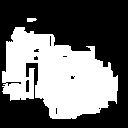
\includegraphics[width=2cm]{figures/results/samples/uncond/sample18_map_floormap_generated.png}
		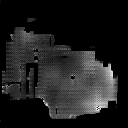
\includegraphics[width=2cm]{figures/results/samples/uncond/sample18_map_heightmap_generated.png}
		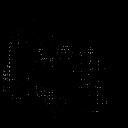
\includegraphics[width=2cm]{figures/results/samples/uncond/sample18_map_thingsmap_generated.png}
		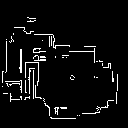
\includegraphics[width=2cm]{figures/results/samples/uncond/sample18_map_wallmap_generated.png}
	\end{center}
	
	\begin{center}
		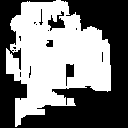
\includegraphics[width=2cm]{figures/results/samples/uncond/sample21_map_floormap_generated.png}
		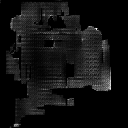
\includegraphics[width=2cm]{figures/results/samples/uncond/sample21_map_heightmap_generated.png}
		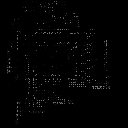
\includegraphics[width=2cm]{figures/results/samples/uncond/sample21_map_thingsmap_generated.png}
		\includegraphics[width=2cm]{figures/results/samples/uncond/sample21_map_wallmap_generated.png}
	\end{center}

	\begin{center}
		\includegraphics[width=2cm]{figures/results/samples/uncond/sample27_map_floormap_generated.png}
		\includegraphics[width=2cm]{figures/results/samples/uncond/sample27_map_heightmap_generated.png}
		\includegraphics[width=2cm]{figures/results/samples/uncond/sample27_map_thingsmap_generated.png}
		\includegraphics[width=2cm]{figures/results/samples/uncond/sample27_map_wallmap_generated.png}
	\end{center}
	
	\begin{center}
		\includegraphics[width=2cm]{figures/results/samples/uncond/sample28_map_floormap_generated.png}
		\includegraphics[width=2cm]{figures/results/samples/uncond/sample28_map_heightmap_generated.png}
		\includegraphics[width=2cm]{figures/results/samples/uncond/sample28_map_thingsmap_generated.png}
		\includegraphics[width=2cm]{figures/results/samples/uncond/sample28_map_wallmap_generated.png}
	\end{center}
	

	
\end{minipage}
\caption[Samples Generated by the Unconditional network (1 of 2)]{Samples generated by the unconditional network (1 of 2). From left to right: Floormap, Heightmap, Thingsmap, Wallmap}
\label{fig:samples-uncond-1}
\end{figure}
\begin{figure}[h!] 
\begin{minipage}[b]{\linewidth}
		\begin{center}
		\includegraphics[width=2cm]{figures/results/samples/uncond/sample31_map_floormap_generated.png}
		\includegraphics[width=2cm]{figures/results/samples/uncond/sample31_map_heightmap_generated.png}
		\includegraphics[width=2cm]{figures/results/samples/uncond/sample31_map_thingsmap_generated.png}
		\includegraphics[width=2cm]{figures/results/samples/uncond/sample31_map_wallmap_generated.png}
	\end{center}
	
	\begin{center}
		\includegraphics[width=2cm]{figures/results/samples/uncond/sample3_map_floormap_generated.png}
		\includegraphics[width=2cm]{figures/results/samples/uncond/sample3_map_heightmap_generated.png}
		\includegraphics[width=2cm]{figures/results/samples/uncond/sample3_map_thingsmap_generated.png}
		\includegraphics[width=2cm]{figures/results/samples/uncond/sample3_map_wallmap_generated.png}
	\end{center}
	
	\begin{center}
		\includegraphics[width=2cm]{figures/results/samples/uncond/sample4_map_floormap_generated.png}
		\includegraphics[width=2cm]{figures/results/samples/uncond/sample4_map_heightmap_generated.png}
		\includegraphics[width=2cm]{figures/results/samples/uncond/sample4_map_thingsmap_generated.png}
		\includegraphics[width=2cm]{figures/results/samples/uncond/sample4_map_wallmap_generated.png}
	\end{center}
	
	\begin{center}
		\includegraphics[width=2cm]{figures/results/samples/uncond/sample6_map_floormap_generated.png}
		\includegraphics[width=2cm]{figures/results/samples/uncond/sample6_map_heightmap_generated.png}
		\includegraphics[width=2cm]{figures/results/samples/uncond/sample6_map_thingsmap_generated.png}
		\includegraphics[width=2cm]{figures/results/samples/uncond/sample6_map_wallmap_generated.png}
	\end{center}
	
	\begin{center}
		\includegraphics[width=2cm]{figures/results/samples/uncond/sample8_map_floormap_generated.png}
		\includegraphics[width=2cm]{figures/results/samples/uncond/sample8_map_heightmap_generated.png}
		\includegraphics[width=2cm]{figures/results/samples/uncond/sample8_map_thingsmap_generated.png}
		\includegraphics[width=2cm]{figures/results/samples/uncond/sample8_map_wallmap_generated.png}
	\end{center}

\end{minipage}
\caption[Samples Generated by the Unconditional network (2 of 2)]{Samples generated by the unconditional network (2 of 2). From left to right: Floormap, Heightmap, Thingsmap, Wallmap}
\label{fig:samples-uncond-2}
\end{figure}

\FloatBarrier
\subsection{Conditional Network}
\paragraph{} 
\begin{figure}[h!] 
	\begin{minipage}[b]{\linewidth}
		
	\begin{center}
		\includegraphics[width=2cm]{figures/results/samples/cond/sample0_map_heightmap_true.png}
		\includegraphics[width=2cm]{figures/results/samples/cond/sample0_map_wallmap_true.png}
		\hfill 
		\includegraphics[width=2cm]{figures/results/samples/cond/sample0_map_floormap_generated.png}
		\includegraphics[width=2cm]{figures/results/samples/cond/sample0_map_heightmap_generated.png}
		\includegraphics[width=2cm]{figures/results/samples/cond/sample0_map_thingsmap_generated.png}
		\includegraphics[width=2cm]{figures/results/samples/cond/sample0_map_wallmap_generated.png}
	\end{center}
	
	\begin{center}
		\includegraphics[width=2cm]{figures/results/samples/cond/sample11_map_heightmap_true.png}
		\includegraphics[width=2cm]{figures/results/samples/cond/sample11_map_wallmap_true.png}
		\hfill 
		\includegraphics[width=2cm]{figures/results/samples/cond/sample11_map_floormap_generated.png}
		\includegraphics[width=2cm]{figures/results/samples/cond/sample11_map_heightmap_generated.png}
		\includegraphics[width=2cm]{figures/results/samples/cond/sample11_map_thingsmap_generated.png}
		\includegraphics[width=2cm]{figures/results/samples/cond/sample11_map_wallmap_generated.png}
	\end{center}
	

	\end{minipage}
\caption[Samples Generated by the Conditional network (1 of 2)]{Samples generated by the Conditional network (1 of 2). In the left column, the heightmap and the wallmap of the \textit{true} level that corresponds to the feature vector used to generate the corresponding level. On the right column, the corresponding generated Floormap, Heightmap, Thingsmap and Wallmap}
\label{fig:samples-cond-1}
\end{figure}

\begin{figure}[h!] 
	\begin{minipage}[b]{\linewidth}
		\begin{center}
		\includegraphics[width=2cm]{figures/results/samples/cond/sample13_map_heightmap_true.png}
		\includegraphics[width=2cm]{figures/results/samples/cond/sample13_map_wallmap_true.png}
		\hfill 
		\includegraphics[width=2cm]{figures/results/samples/cond/sample13_map_floormap_generated.png}
		\includegraphics[width=2cm]{figures/results/samples/cond/sample13_map_heightmap_generated.png}
		\includegraphics[width=2cm]{figures/results/samples/cond/sample13_map_thingsmap_generated.png}
		\includegraphics[width=2cm]{figures/results/samples/cond/sample13_map_wallmap_generated.png}
	\end{center}

	\begin{center}
		\includegraphics[width=2cm]{figures/results/samples/cond/sample17_map_heightmap_true.png}
		\includegraphics[width=2cm]{figures/results/samples/cond/sample17_map_wallmap_true.png}
		\hfill 
		\includegraphics[width=2cm]{figures/results/samples/cond/sample17_map_floormap_generated.png}
		\includegraphics[width=2cm]{figures/results/samples/cond/sample17_map_heightmap_generated.png}
		\includegraphics[width=2cm]{figures/results/samples/cond/sample17_map_thingsmap_generated.png}
		\includegraphics[width=2cm]{figures/results/samples/cond/sample17_map_wallmap_generated.png}
	\end{center}
	
	\begin{center}
		\includegraphics[width=2cm]{figures/results/samples/cond/sample1_map_heightmap_true.png}
		\includegraphics[width=2cm]{figures/results/samples/cond/sample1_map_wallmap_true.png}
		\hfill 
		\includegraphics[width=2cm]{figures/results/samples/cond/sample1_map_floormap_generated.png}
		\includegraphics[width=2cm]{figures/results/samples/cond/sample1_map_heightmap_generated.png}
		\includegraphics[width=2cm]{figures/results/samples/cond/sample1_map_thingsmap_generated.png}
		\includegraphics[width=2cm]{figures/results/samples/cond/sample1_map_wallmap_generated.png}
	\end{center}
	
	\begin{center}
		\includegraphics[width=2cm]{figures/results/samples/cond/sample21_map_heightmap_true.png}
		\includegraphics[width=2cm]{figures/results/samples/cond/sample21_map_wallmap_true.png}
		\hfill 
		\includegraphics[width=2cm]{figures/results/samples/cond/sample21_map_floormap_generated.png}
		\includegraphics[width=2cm]{figures/results/samples/cond/sample21_map_heightmap_generated.png}
		\includegraphics[width=2cm]{figures/results/samples/cond/sample21_map_thingsmap_generated.png}
		\includegraphics[width=2cm]{figures/results/samples/cond/sample21_map_wallmap_generated.png}
	\end{center}
	
	\begin{center}
		\includegraphics[width=2cm]{figures/results/samples/cond/sample26_map_heightmap_true.png}
		\includegraphics[width=2cm]{figures/results/samples/cond/sample26_map_wallmap_true.png}
		\hfill 
		\includegraphics[width=2cm]{figures/results/samples/cond/sample26_map_floormap_generated.png}
		\includegraphics[width=2cm]{figures/results/samples/cond/sample26_map_heightmap_generated.png}
		\includegraphics[width=2cm]{figures/results/samples/cond/sample26_map_thingsmap_generated.png}
		\includegraphics[width=2cm]{figures/results/samples/cond/sample26_map_wallmap_generated.png}
	\end{center}
	
	\begin{center}
		\includegraphics[width=2cm]{figures/results/samples/cond/sample27_map_heightmap_true.png}
		\includegraphics[width=2cm]{figures/results/samples/cond/sample27_map_wallmap_true.png}
		\hfill 
		\includegraphics[width=2cm]{figures/results/samples/cond/sample27_map_floormap_generated.png}
		\includegraphics[width=2cm]{figures/results/samples/cond/sample27_map_heightmap_generated.png}
		\includegraphics[width=2cm]{figures/results/samples/cond/sample27_map_thingsmap_generated.png}
		\includegraphics[width=2cm]{figures/results/samples/cond/sample27_map_wallmap_generated.png}
	\end{center}
	
	\begin{center}
		\includegraphics[width=2cm]{figures/results/samples/cond/sample29_map_heightmap_true.png}
		\includegraphics[width=2cm]{figures/results/samples/cond/sample29_map_wallmap_true.png}
		\hfill 
		\includegraphics[width=2cm]{figures/results/samples/cond/sample29_map_floormap_generated.png}
		\includegraphics[width=2cm]{figures/results/samples/cond/sample29_map_heightmap_generated.png}
		\includegraphics[width=2cm]{figures/results/samples/cond/sample29_map_thingsmap_generated.png}
		\includegraphics[width=2cm]{figures/results/samples/cond/sample29_map_wallmap_generated.png}
	\end{center}
	
	\begin{center}
		\includegraphics[width=2cm]{figures/results/samples/cond/sample2_map_heightmap_true.png}
		\includegraphics[width=2cm]{figures/results/samples/cond/sample2_map_wallmap_true.png}
		\hfill 
		\includegraphics[width=2cm]{figures/results/samples/cond/sample2_map_floormap_generated.png}
		\includegraphics[width=2cm]{figures/results/samples/cond/sample2_map_heightmap_generated.png}
		\includegraphics[width=2cm]{figures/results/samples/cond/sample2_map_thingsmap_generated.png}
		\includegraphics[width=2cm]{figures/results/samples/cond/sample2_map_wallmap_generated.png}
	\end{center}
	
	\begin{center}
		\includegraphics[width=2cm]{figures/results/samples/cond/sample30_map_heightmap_true.png}
		\includegraphics[width=2cm]{figures/results/samples/cond/sample30_map_wallmap_true.png}
		\hfill 
		\includegraphics[width=2cm]{figures/results/samples/cond/sample30_map_floormap_generated.png}
		\includegraphics[width=2cm]{figures/results/samples/cond/sample30_map_heightmap_generated.png}
		\includegraphics[width=2cm]{figures/results/samples/cond/sample30_map_thingsmap_generated.png}
		\includegraphics[width=2cm]{figures/results/samples/cond/sample30_map_wallmap_generated.png}
	\end{center}
		
		
	\end{minipage}
	\caption[Samples Generated by the Conditional network (2 of 2)]{Samples generated by the Conditional network (2 of 2). In the left column, the heightmap and the wallmap of the \textit{true} level that corresponds to the feature vector used to generate the corresponding level. On the right column, the corresponding generated Floormap, Heightmap, Thingsmap and Wallmap}
	\label{fig:samples-cond-2}
\end{figure}


\section{Results Evaluation}
\label{sec:results-evaluation}
\paragraph{} We conduct the analysis of the results in the same order as they are presented in the previous sections, eventually making reference to content which is included in the Appendix. The first part of our discussion considers the metrics that have been monitored during the training phase, explaining the results. After that, we consider the results of the experiments described in section \ref{sec:experiments}.
\subsection{Sample Evaluation Metrics}
\paragraph{} Training losses in figures \ref{fig:train-cond-loss} and \ref{fig:train-uncond-loss} confirm the advantages of the WGAN model over earlier proposals, it is indeed possible to appreciate a converging behaviour similar to that of classical Neural Networks in both the conditional and unconditional case. This proved to be useful for understanding when to stop the training phase, since a manual inspection of the samples wouldn't be informative of the actual network capabilities. The fact that the validation loss follows the behaviour of the training loss also suggests a good generalization capability of the critic in assigning level scores even for previously unseen samples. 

\paragraph{} Entropy Mean Absolute Errors in figure \ref{fig:train-entropy-mean} converge toward a small value in the same way the loss does, confirming that the WGAN loss is actually correlated to the sample quality in our case. In particular this metric is related to the difference in information content, or noise, between true and generated samples. While a small difference is still detectable, both networks showed to reduce this difference as the training proceeded.

\paragraph{} Mean Structural Similarity (Figure~\ref{fig:train-similarity}) shows that the conditional network generates samples that are structurally more similar to true levels than the unconditional network does. This is also true if we consider the networks in their early training stage. It's worth nothing that the structural similarity is a metric for evaluating the perceived sample quality, so it reaches unitary values only if the two samples are the same. In our setting we compare different levels so we cannot treat SSIM as an absolute value but only as an indicator of the "relative quality" of the samples generated by the two networks.

\paragraph{} Encoding Error in figures \ref{fig:train-encoding_error-floormap} to \ref{fig:train-encoding-error-thingsmap} shows that the network is capable to easily learn and reproduce the colour coding used in each separated map. This does not mean that the network is able, for example, to only output either the value 0 or 255 when generating a floormap, but this metric shows that the average error is small. For this reason, the only post-processing we apply to generated samples in order to compute the generated features is to threshold the colour value toward the closest meaningful value (eg. a 244 in a floormap is interpreted as a 255). 

\paragraph{} Corner Error in figures \ref{fig:floor_corner_error} and \ref{fig:wall_corner_error} shows that while the unconditional network generates levels that don't significantly improve their corner count with respect to the true ones, the conditional network actually learns to generate more accurate levels. This value could hardly reach low values as two levels having the same features (with reference to the ones we have selected as inputs) could naturally differ in their topology, raising the value of this metric. Another aspect that is worth nothing is the lower variance in the conditional case, possibly reflecting a lower amount of noise or artefacts in generated levels.

\clearpage

\subsection{Experiments Discussion}
\paragraph{} The first columns of tables \ref{tab:results-input-features} and \ref{tab:results-other-features} show for what features it is not possible to reject the hypothesis that the true distribution and the distribution generated by the unconditional network are equal. If we analyse these features we can notice that many features that are "well learned" by the network in their output depend on the level area or the perimeter. In particular, figure \ref{fig:results-input-features} and \ref{fig:results-input-distr-features} show how the two networks are able to reproduce the level area distribution (level\_equivalent\_diameter) and the length of the minor axis of the levels. 

\paragraph{} The second column of the tables shows the same concept for the conditional network. In particular, table \ref{tab:results-input-features} shows substantial improvements on the input features: In this case, the feature  \textit{distmap-kurt} (associated to the "variety" in room dimensions), is now distributed enough closely to the real distribution that the null hypothesis cannot be rejected any more. The input features that have been learned by the unconditional network are also learned by the conditional network. For the features \textit{solidity, nodes (number of rooms)} and \textit{distmap skewness (balance between big and small areas)} the conditional network cannot reproduce a distribution that is close enough to the real one to change the outcome of the test, however the statistic values in table~\ref{sec:app-ks} indicate that the distributions of the conditional network are the closest to the real one~\footnote{This fact is also indicated with an asterisk in table \ref{tab:results-input-features}}.

\paragraph{} If we analyse the results in table \ref{tab:results-other-features} and graphs in Appendix~\ref{sec:appendix-graphs} we can confirm in many case the behaviour stated in the previous paragraph: features which are better represented by both networks (group F3) are related with the levels area. Features expressing  locations of particular points of the maps such as the topological centroid or even explicitly represented as the player starting point, are unsurprisingly not well represented by the networks. The features regarding the number of items in the level, which would be useful from a design point of view, are still not well represented probably due to the still too high presence of checker board artefacts in the \textit{Thingsmap}. However, the conditional proved again to be the best of the two networks in describing this set of features, learning particularly well with the distribution of "power-ups". The last set of listed features is, as expected, not well learned by the networks since it is composed by features which are graph-metrics or other too complex features, for which this kind of model is not suitable.

\paragraph{} Graphs of figure~\ref{fig:results-exp3-features} show how the unconditional network response varies by changing each input features to the values that correspond to the three quartiles of the true distribution. Even if in no cases the input feature can deterministically control the output feature of the value, for the majority of features it is possible to alter the output distribution by acting on the input value. This fact is represented by the ordering of the curves, in many case reflecting the ordering of requested values.
In particular we can notice how all the features except the \textit{solidity} and \textit{distmap-kurt} react well to values changes. The particular shape of some curves such in \textit{distmap-kurt} and \textit{major axis} may suggest that the location of the output features does not linearly follow the translation of the requested feature or it could work as intended only in some areas of feature space. The particular undesired behaviour of the 75th percentile of \textit{level solidity} can be due to the network failing to learn the representation of such high \textit{solidity} values, or the presence of many artefacts in the corresponding generated levels leading to a incorrect calculation of the feature. 
It is worth noting that due to the sampling issues we considered in the previous chapters, this experiment has been conducted by selecting different feature vectors that exhibited the desired value on a particular feature. The possible drawback of this experiment is that the visualized distributions could depend on other factors other than the single requested feature value, however we observed better or similar results in earlier networks we trained with different settings, suggesting that the issue we just highlighted could have marginal impact on our results.


\subsection{Visual Acknowledgement}
\paragraph{} The results we discussed in the earlier sections indicate that the conditional network has some advantages over the unconditional version, which can be briefly resumed as a better overall sample quality (Sample Evaluation Metrics), a better learning of input and other topological features (experiments 1 and 2) and the possibility to control the level generation up to some extent (Experiment 3). In a last consideration about these results we want to highlight that our experiments focused on proving the ability of the networks to reproduce the true feature distributions of the original dataset. This means that if the null hypothesis for one feature cannot be rejected then we can assume that its distribution may be "close enough" to the true one to generate levels which are similar to the existing ones. The contrary, however, does not necessarily prevents the model to be effectively used as a tool for generating levels, but only indicates that the generated levels somehow differs from the true ones. This fact can be appreciated by a visual comparison of the true and generated samples we proposed in section~\ref{sec:samples}: in many cases it is possible to notice that the global shape and size of the generated samples vaguely resembles that of the true levels, indicating that the network actually considers some of the requested features up to a certain point. On the same figure it is possible to notice some struggle of the network in representing smaller features such level borders, probably due to generation noise. This can alter the calculated features and lead to inaccurate distributions, for this reason we recommend to apply some morphological processing or noise reduction techniques before converting the generated images to playable WAD files in order to reduce the generation noise.



\section{Summary}
\paragraph{} In this chapter we presented our results by first showing the quality difference in samples generated by the two networks, according to the evaluation metrics defined in section \ref{sec:evaluation} and then showing experimental results for testing the relation between the true and generated features and the impact of the input features in the conditional network. For providing a visual comparison of the generated levels, we also showed a set of generated samples for each network. In the last section we discussed in detail our results by first analysing the sample evaluation using evaluation metrics, then by considering the results of the experiments that analyse the networks behaviour with respect to the input features. In the next chapter, we provide more general considerations about our work and highlight the open problems and the possible future works.